\section{Korisnički interfejs}

Korisnički interfejs za desktop aplikaciju. Korišćeni alati su javaFX i Scene Builder. Konkretno je prezentovan interfejs za rad sa ponudama.

Početni ekran predstavlja autentifikaciju, koja je deo popratne komponente sistema. Neophodno je administrator da doda novog korisnika u bazu, čime je omogućeno logovanje korisnika. Nalog korisnika aplikacije ima sopstveni nalog za konekciju ka bazi podataka. Radi evedenicije izmena fajlova.

[Prototip: samo pritisnuti potvrdi za dalji korak]

\begin{figure}[ht]
\centering
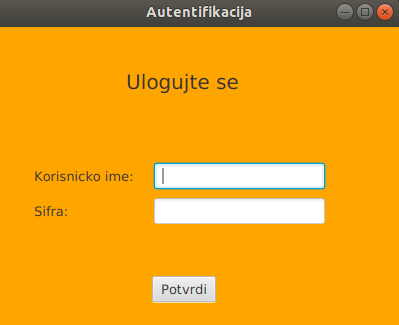
\includegraphics{slike/UI-1.png}%
\caption{Autentifikacija}
\end{figure}

\clearpage

Autentifikacijom vrši se i autorizacija, koja nudi korisniku module poslavanja kojima on ima pravo pristupa, na osnovu zaduženja u firmi.

[Prototip: nudi samo modul prodaja]

\begin{figure}[ht]
\centering
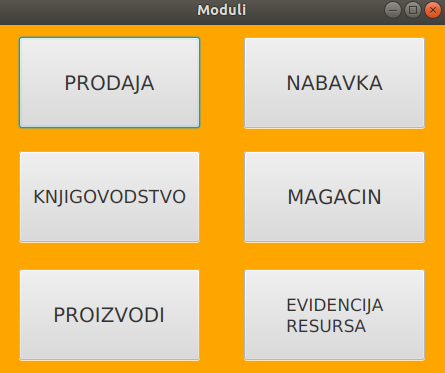
\includegraphics{slike/UI-2.png}%
\caption{Početni meni sa doyvoljenim pristupima}
\end{figure}

\clearpage

Sektor prodaje sadrži pod-sektore za izradu potrebnih dokumenata.

[Prototip: nudi pod-sektor ponude]

\begin{figure}[ht]
\centering
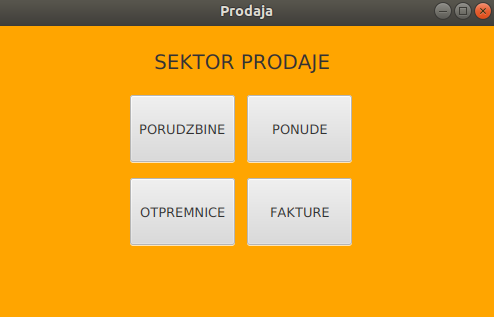
\includegraphics[width=165mm]{slike/UI-3.png}%
\caption{Sektor za prodaju}
\end{figure}

\clearpage

Odabirom ponude, prikazuje se interfejs za njihovo korišćenje. 

Dugme Učitaj ponude prikazuje sve ponude iz baze, kao i dodatne informacije o njima. Recimo kada je poslednja izmena izvršena i koji korisnik je to uradio.

Dugme Dodaj novu, prikazuje novi interfejs slican narednom za izmene ponuda i omogućuje dodavanje novog dokumenta ponuda.
[Prototip: samo funkcioniše popunjavanje id porudžbine]

Dugme obriši, briše ponudu čiji je id unet u polje iznad.

Dugme Izmeni ponudu, prikazuje interfejs sa naredne slike za ponudu ciji je id unet u polje iznad dugmeta.

\begin{figure}[ht]
\centering
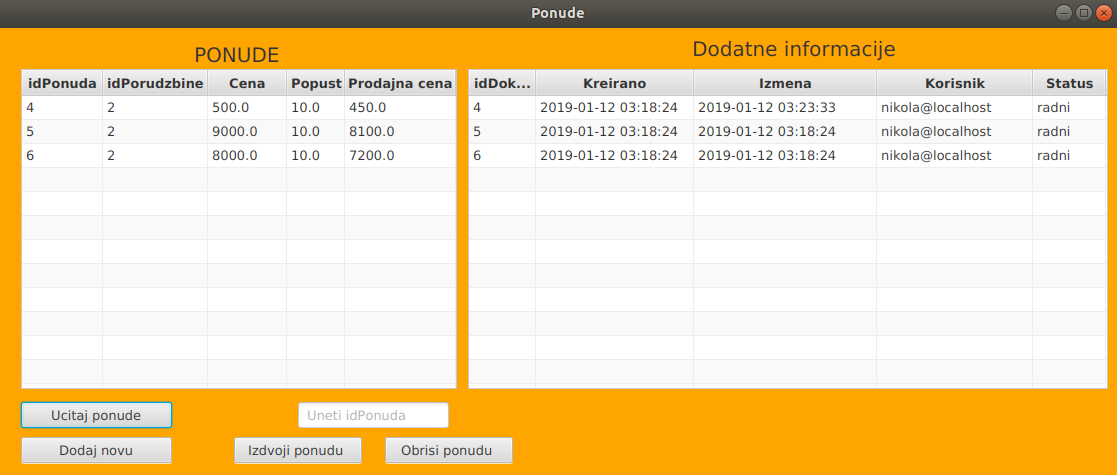
\includegraphics[width=165mm]{slike/UI-4.png}%
\caption{Prikaz ponuda}
\end{figure}

\clearpage

Interfejs za izmenu ponuda prikazuje informacije vezane za nju, kao i stavke koje ponuda sadrži.
Dugme izmeni čuva nove informacije u bazu.
Promene pozivaju trigere iz baze, pa tako menjanje popusta automatski menja i prodajnu cenu.

[Prototip: samo popust se može menjati]

Spikas stavki, moguće je menjati dodanvanjem dovih ili brisanjem starih. Cena se ne unosi već se automatski formira iz cene proizvoda i količini. Dodavanjem stavki menja se i cena ponude.


\begin{figure}[ht]
\centering
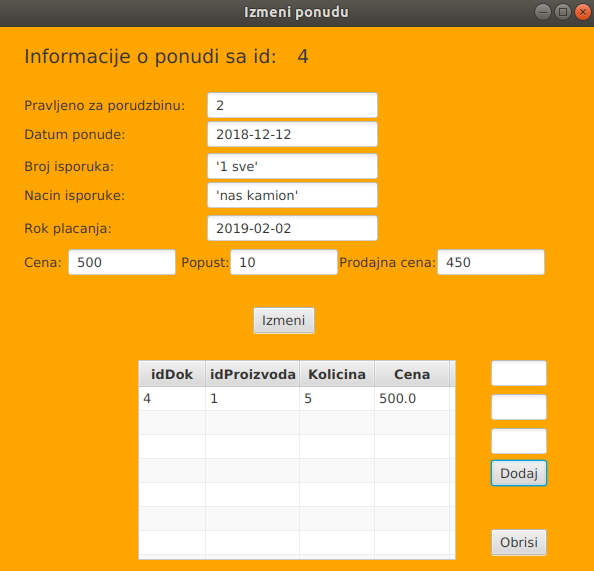
\includegraphics[width=165mm,height=130mm]{slike/UI-5.png}%
\caption{Izdvojena ponuda}
\end{figure}
